% Latex main.tex file for Xiaochuan Tian's Master Thesis at the University of Memphis
% Advisor: Dr. Eunseo Choi
% Date: 2015,February ~ April
% Location: Center for Earthquake Research and Information
% Title: 3D Numerical Models for Along-axis Variations in Diking at Mid-Ocean Ridges
% The format and structure according to: Thesis requirements from the University of Memphis: 
% http://www.memphis.edu/gradschool/tdinfo_electronic.php#samplepages (referred as RQ(Requirements) in the code)
% <> is refered as a symbol for question or problem needed to be answered or solved
% Samples of recent submitted Thesis can be found from:
% https://umwa.memphis.edu/etd/

%%-----------------------------------------------------
%% Thesis Environments Setup
%%-----------------------------------------------------

\documentclass[12pt]{article}  % RQ 3.1

\usepackage{times}             % RQ 3.1 (this is not exactly times new roman but very similar)
\usepackage[top=1.0in, right=1.0in, bottom=1.0in, left=1.5in]{geometry} % RQ 3.2
% <> RQ 3.2 0.5inches for page numbers postistion haven't been added
\usepackage{setspace}
\doublespacing                 % RQ 3.4
\renewcommand{\contentsname}{\textit{\small{Table of Contents}}}  % Change from Contents to Table of Contents
\usepackage{hyperref}    % For hyperlinks to contents
\usepackage{natbib}  %for \citep

\usepackage{graphics}
\usepackage{epsfig}

\usepackage{amsmath}
%\usepackage{float}  % for floating figures
\usepackage{floatrow} %for caption of figures on its side
\usepackage{gensymb} %for \degree
\usepackage{subcaption} %for figures side by side

\usepackage{diagbox} % for table cell with a diagonal line and 2 sub cells

%\setcounter{secnumdepth}{5} %for \paragragh
%%------------------------------------------------ 
% For trackchanges.sty  (For co-revision)
% Change the editor name as you like         
%%------------------------------------------------
\usepackage[inline]{trackchanges}
\addeditor{XT}
\addeditor{EC}
%%------------------------------------------------
% Try one of these commands:
%     \add[editor]{added text}
%     \remove[editor]{removed text}
%     \change[editor]{removed text}{added text}
%     \note[editor]{note text}
%     \annote[editor]{text to annotate}{note text}
%%------------------------------------------------   

%%-------------------------------------------------
% \includeonly files that have been made changes for 
%     faster processing during revision processes
%%-------------------------------------------------

% Uncomment the following line will process the whole file.

\includeonly{Title_Page, Copyright_Notice, Dedication, Acknowledgements, Abstract, Table_of_Contents, Introduction, Methods, Results, Discussion, Conclusions}

% Comment the previous line and type below the chapter you are frequently making changes.

%\includeonly{Results}

%%-----------------------------------------------------
%% Thesis Begin
%%-----------------------------------------------------

\begin{document}

%%--------------------------------------------------
% Preleminary Pages
%%--------------------------------------------------
\pagenumbering{roman}


\thispagestyle{empty}  % For hiding the page number at the title page

\newgeometry{top=2.0in, left=1.5in}

\begin{center}


\uppercase{3D Numerical Models for Along-axis Variations in Diking at Mid-Ocean Ridges}
\\
\vspace{10pt}
by
\vspace{10pt}
\\
Tian, Xiaochuan
\\
\begin{CJK}{UTF8}{gbsn}
田小川
\end{CJK}
\\
\vspace{100pt}

A Thesis
\\
%\vspace{2pt}
Submitted in Partial Fulfillment of the 
\\
%\vspace{2pt}
Requirements for the Degree of 
\\
%\vspace{2pt}
Master of Science
\\
\vspace{35pt}

Major: Earth Sciences
\\

\vspace{120pt}

The University of Memphis
\\

August, 2015

\end{center}

\restoregeometry

\begin{center}
  \vspace*{\fill}
Copyright \copyright \ 2015 Xiaochuan Tian
\\All rights reserved
  \vspace*{\fill}
\end{center}
 % optional
\begin{center}
\textbf{\textit{Dedication}}
\end{center}

I would like to dedicate this thesis to my mother, Xia Tian. I wouldn't have a chance to experience this wonderful world without her giving birth to me. She rears me up by herself with her great love, optimism and peseverence. Without her guidance and support, I will not become who I am.

I also want to dedicate this thesis toward my major thesis advisor: Dr. Eunseo Choi. His mentorship defines what a great advisor is like. Without his  guidance, neither this theis nor my fast personal-development during these two years is possible. He has kindled a flame that illuminates the way for my future career as a geodynamic modeler.   

 % optional
\begin{center}
\textbf{\textit{\large{Acknowledgements}}}
\end{center}

There is no proper words for me to express my deep gratitude toward my thesis advisor, Professor Eunseo Choi. He has changed my life in a very positive way. From him, I have learned what a great researcher and educator should be like. It is because of his unfailing care and understanding that have given me the courage to persevere, and to carry on during the darkest days as an international student far away from home. It is his vivid and interesting lessons that have inspired me so much that I want to devote my career into geodynamic modeling. It is his numerous inspiration and encouragement that has motivated me to work super hard (enjoy at the same time) on the fascinating research questions. It is his altruistic share that has provided me with great chances to learn from outstanding researchers, references, and to attend meetings. It is his patience to guide me through my endless silly questions that has nurished and cultivated my capabilities of being an independent researcher. Blessings from Eunseo, my role model, are countless. I will keep them in mind and try my best to relay the torch.
\\
I would also like to thank members of my thesis committee, Professor Christine Powell and Professor Jer-Ming Chiu, for their guidance and support. Especially I want to thank Dr. Chiu for his sharing and advice on my course term projects and for his patience to answer all my silly questions. In addition, I want to thank Dr. Powell for your warmhearted encouragement and benevolence during my studies at the Center for Earthquake Research and Information (CERI). 
\\
My sincere thanks must also go to the CERI and the University of Memphis (UM). Thanks a lot for providing me this great chance to study here with full tuition and graduate research assistanship. It is this kind support that has made my two-year studies at this great institution possible. 
\\
I am also grateful to the courses instructors for many vivid and interesting courses that have stimulated my interests in Geophysics, helped me build up my foundation and expanded my horizon in the field. They are Professor Robert Smalley for ``Data Analysis in Geophysics'', Professor Charles Langston for ``Global Seismology'' and ``Inverse Methods in Geophysics'', Professor Mitch Withers for ``Signal Processing in Earth Science'', Professor Eunseo Choi for ``Global Geophysics'' and ``Geodynamics'', Professor Christine Powell for ``Evironmental Geophysics'', Professor Randy Cox for ``Art of Earth Science'', Professor Jer-Ming Chiu for ``Exploration Seismology''. Thank you so much. Especially, I want to thank Professor Withers for you encouragement and your time and efforts for answering all my questions. I would also like to thank Professor Eric Daub for your delicious homemade cakes provdided to us graduate students every Wednesday during the ``CERI Discussion''. I am probably the person who ate the most of them and enjoyed the most.
\\
Many thanks must also go to my dear classmates and research colleagues, with whom, I have lived, studied and worked during the two years. Especially, I want to thank Yang Yang for your supportive help and share on my term projects. Thank you for being a wonderful roommate. I would also like to thank my best ``cubic office mate'', Naeem Khoshnevis, for his best company. We've been studied together as the most diligent (long staying) people in CERI (12/7). Thank you for those benevolent and uncountable ``how are you'', ``good morning'', ``good night'' as well as many good chats. My sincere thanks must also go to Sabber Ahamed, who has been encouraging me during my darkest days when I lost direction. It is his enthusiastic share and encouragement that have helped me go through the bad days. 
\\
Many thanks must also go to CERI staffs. Thank you Chris McGoldrick for many of your kindly help and all the nice chats, from which I have learned many new English words and phrases. Thank you Tanya Broadbent and Kathleen Tucker for sending me birthday gifts which makes me feel so warm as being a member of CERI families. Thank you Christy Chiu and Jer-Ming Chiu for inviting me to your house for Chineses Spring Festival lunch which helped a lot in soothing my nostalgia for hometown. Thank you Gary Patterson for your share and benevolence. Thank you Deshone Marshall for constantly helping me out in using CERI's lab computers. Thank you Josephine Calhoun for providing us tidy and enjoyable environments for studying and doing research everyday. 
\\
I also want to sincerely thank Center for Writing and Communication of the UM. Especially, I want to thank Bill Schraufnagel for your very supportive helps on revising this thesis and enhancing the presentation.
\\
I am also thankful to many great researchers that have encouraged and inspired me for this research. Thank you Professor Lin, Jian for your encouragement during 2014 AGU fall meeting. Thank you Jean-Arthur Olive for your feedback and your kind share. Thank you Professor Taras Gerya for your feedback and your great book \textit{Introduction to Numerical Geodynamic Modelling} that has inspired me a lot. Thank you Professor Suzanne Carbotte for your share and encouragement. Thank you Professor Roger Buck for several inspiring talks and sharing as well as feedbacks on this research.
\\
I also want to thank Professor Liu, Jie (\begin{CJK}{UTF8}{gbsn}刘洁\end{CJK}) and Professor Zhang, Ke (\begin{CJK}{UTF8}{gbsn}张珂\end{CJK}) from Sun Yat-sen University, for kindly sharing your computing resourses on Tianhe2 to me. Many thanks must also go to the staffs of Penguin, Stampede and Tianhe2 supercomputer centers, thank you so much for all the technical supports. Especially, I would like to thank National Supercomputer Center in Guangzhou, China, for providing me surpports with more than 200k of core-hours. 
\\
Sincere thanks must also go to the lifeguards and staffs of the swimming pool of the UM Recreation Center. Thank you for your work in providing me such a safe and enjoyable workout environments. Thank you for accompanying me almost everyday and making sure my safty during I am swimming. I could not endure all the stresses from the high pressure school works if without being able to enjoy swimming everyday.  
\\
In addition, I also want to express my sincere thank to Professor Cheng, Gu (\begin{CJK}{UTF8}{gbsn}成谷\end{CJK}), my undergraduate thesis advisor. Thank you for providing me a chance to start my career as a geophysicist. Thank you for all your guidance and share. 
\\
I should never forget my deep gratitude to my middle school Math teacher Feng, Yan (\begin{CJK}{UTF8}{gbsn}冯艳\end{CJK}) and high school Math teacher Chen, Shengfang (\begin{CJK}{UTF8}{gbsn}陈胜方\end{CJK}) and Physics teacher Lyu, Lijie (\begin{CJK}{UTF8}{gbsn}吕黎洁\end{CJK}) as well as English teacher Cindy (\begin{CJK}{UTF8}{gbsn}叶晓靖\end{CJK}). It is your great education, inspiration, love and care that have cultivated me into a person, who begins able to appreciate the fascinating science world. Your great efforts and patience in teaching me and answering my silly questions have helped me build up a good foundation for my future studies as a science major student.
\\
Special thanks must also go to a special person, Zhang, Siwan (\begin{CJK}{UTF8}{gbsn}张思婉\end{CJK}). Thank you for planted a seed of love and beauty deeply in my heart that has been encouraging and inspiring me through time.    
\\
Finally, I want to thank my families. There simply is no proper word for expressing my gratitude. Thank you so much my dear grandfather Tian, Shengheng (\begin{CJK}{UTF8}{gbsn}田升恒\end{CJK}), and grandmother Wang, Defen (\begin{CJK}{UTF8}{gbsn}王德芬\end{CJK}), who have reared me up with great love and care. Thank you so much my grandgrandfather Tian, Guangzong (\begin{CJK}{UTF8}{gbsn}田光宗\end{CJK}). I will never forget your last words for encouraging me to be a good person and a diligent student.

Thank you my dear mother, Tian, Xia (\begin{CJK}{UTF8}{gbsn}田霞\end{CJK}). You are always a great mother to me. Thank you so much for rearing me up by yourself with your great courage, optimism, love and care. Without you, there is no me.
 % optional
%\include{Preface} % optional
\begin{center}
\textbf{\textit{Abstract}}
\end{center}

\vspace{0.5cm}

\begin{singlespace*}
Tian, Xiaochuan. M.S. The University of Memphis. May 2015 Master of Science. 3D Numerical Models for Along-axis Variations in Diking at Mid-Ocean Ridges. Major Professor: Eunseo Choi.
\end{singlespace*}

\vspace{0.5cm}

Bathymetry of ocean floors reveals a great variety of morphologies at Mid-ocean Ridges (MORs). Previous studies showed that the morphologies at slow spreading MORs are mainly controlled by the ratio between rates of magma supply and plate extension. 2D models for the across-ridge cross-sections have been successful in explaining many of the observed morphological features such as abyssal hills and oceanic core complexes. However, the magma supply varies along the ridge and the interaction between the tectonic plates and magmatism at MORs are inevitably 3D processes. We propose to investigate the consequences of the along-axis variability in diking in terms of faulting pattern and the associated structures. This work will include implementation of an algorithm of parameterizing repeated diking in a 3D parallel geodynamic modeling code.



\begin{center}
  {\hypersetup{hidelinks}
    % the {\hypersetup{hidelinks}
    % } is for hiding the color of the table of content
    \tableofcontents
    \addtocontents{toc}{{Chapter}}
    \addtocontents{toc}{~\hfill{Page}\par}
  }
\end{center}

%\begin{center}
        \listoftables
\end{center}

 % for 5 or more
%\begin{center}
  {\hypersetup{hidelinks}
  \listoffigures
  }
\end{center}

 % for 5 or more
%\include{Key_to_Symbols_or_Abbreviations} % optional

%%--------------------------------------------------
% Text
%%--------------------------------------------------
\pagenumbering{arabic}

\pagebreak
\section{Introduction}
\label{ch:Intro}  % <>? why ch: befor Intro

\subsection{Research Questions}
\subsection{Review of Literature}
\subsection{Statement of Research Purpose}
\subsection{Findings}


\pagebreak
\section{Methods}
\label{ch:Methods}

\subsection{Method of approach}
\subsection{Model Setup}
\subsection{Parameters to control}

\pagebreak
\section{Results}

Currently, we have three factors controlling the model behaviors. They are three ranges of M variation along the ridge axis (0.5$\sim$0.7; 0.5$\sim$0.8; 0.2$\sim$0.8), three functional forms of M variation (linear; sinusoidal; square root) and two types of weakening rate (Type 1 and Type 2) as mentioned in Parameters to control section. Generally, all models forms a median valley that deepens and widens toward the lower M side. 

\subsection{Reference model description}
We consider two models as our reference models: one, M varies linearly from 0.2 to 0.8 along the ridge axis; two, constant M along the ridge axis as a comparison to the varying M models.

\subsubsection{M varies along the ridge axis}

\begin{figure}[H]
  \centering
    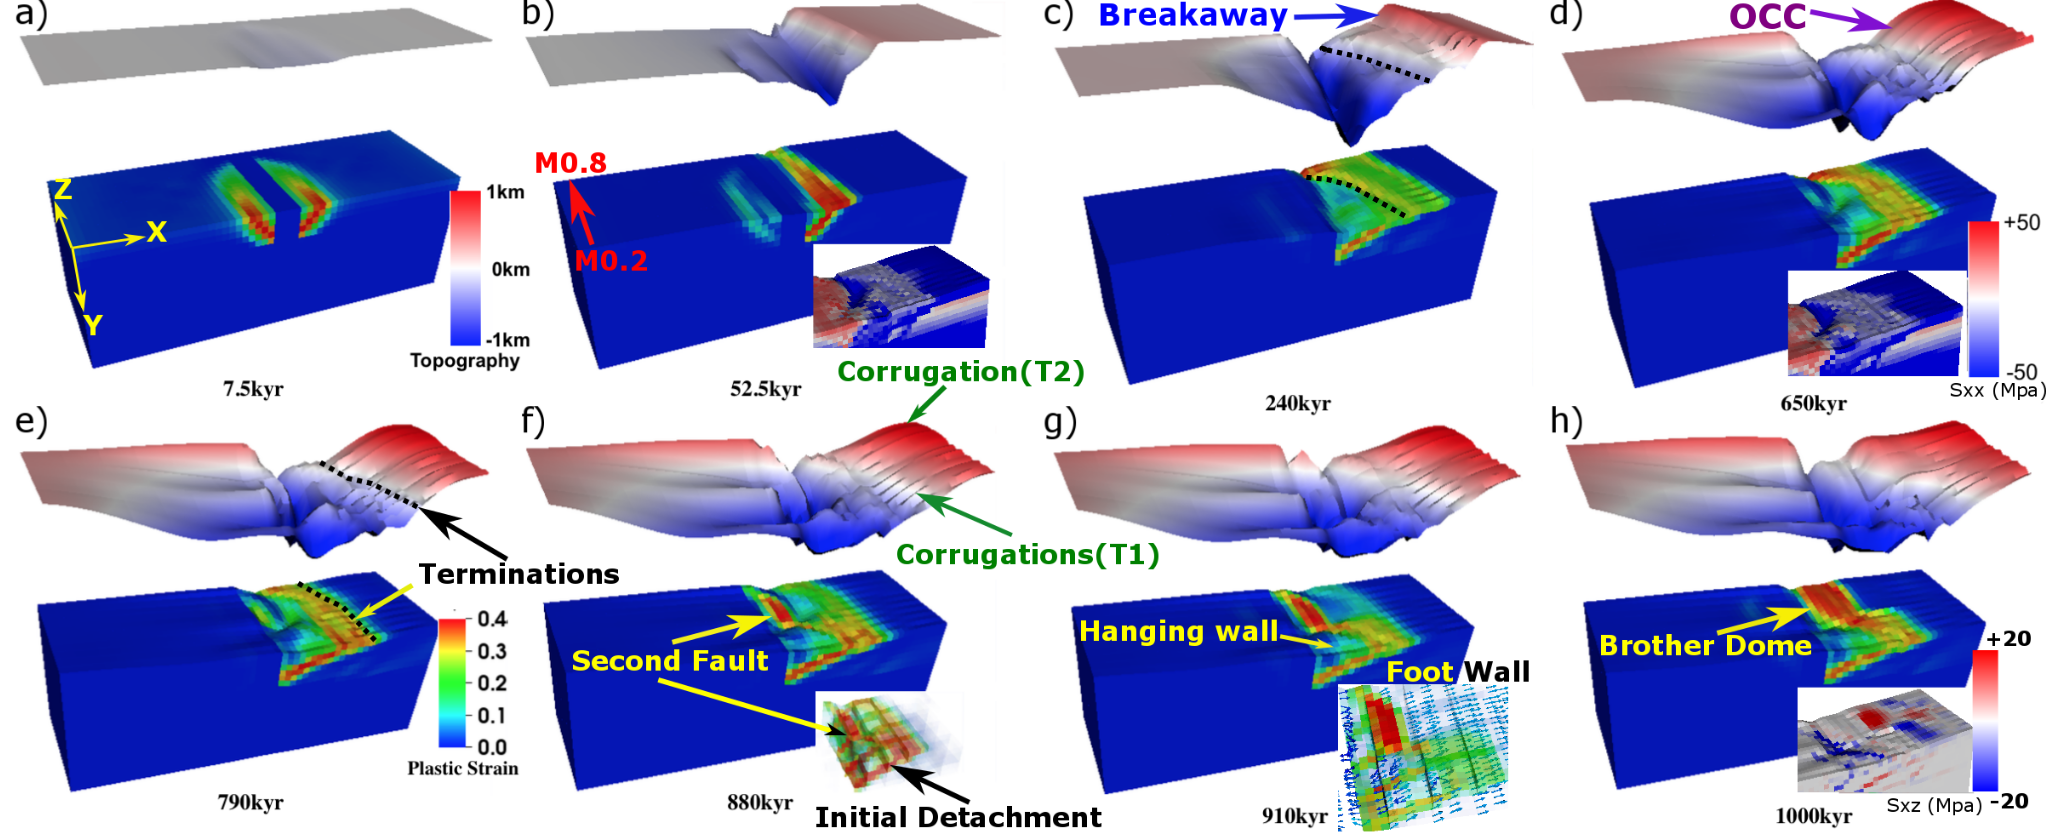
\includegraphics[width=1.0\textwidth]{fig_Results1_1.png}
  \caption{Reference model one: M linearly increases from 0.2 to 0.8 from front to back. The top layer is the topography of the model with five times vertical exaggeration. The green, yellow and red colors shown in the model domain are for Plastic strain. The number with kyr beneath is the time for the model with a unit of thousands of year. The two insets for 650kyr and 1000kyr is for shear stress $\sigma_{xz}$ (Sxz in the figure). The inset for 880kyr is for plastic strain. The inset for 910kyr shows both plastic strain and the velocity vector.} %\note[XT]{one thing to be noted is that the $dt=0.5yr$ in these series of 3D models, thus I divided the time step by two to get the time (kyr). This figure needs to be revised that the plastic strain scale is actually changing for different time, a way to revise it is to maintain a constant color scale or attach a color scale for each time. Also, it seems a little bit small and two rows is not as preferable as one row or one column to better express the concept of linear time series evolution.}}
 \label{fig_Results1_1}
\end{figure}   

As shown in Figure~\ref{fig_Results1_1}, at 7.5kyr, high angle normal faults (shown as high plastic strain shear bands) begin to form near the ridge axis because the thickness of the crust is thinnest at the ridge center according to model thermal structure. They first initiate at the front (lower M side) and then nucleate to the back (higher M side) because for each timestep, the tensional stress accummulates more at the lower M side and thus reach a yielding point earlier than higher M side. At 52.5kyr, the normal fault on the right hand side of the ridge axis continues to evolve while the one on the left becomes inactive. The choice of which fault will delvelop is a random event since the model setup is symmetrical across the ridge-axis. The timing difference of initiation of faulting along the ridge axis create a constant offset in X-axis direction of breakways that the breakaway at the lower M side extends further than that of the higher M side. However, this offset will not increase because the velocity for the breakaway to move away from the axis is only controlled by the far field extension rate, $V_{x}$.
%the fault displacement at the front side is larger than that of the back because M is lower at the front and more extension needed to be accommodated by the tectonic processes (i.e. normal faulting). \annote[XT]{Thus, the breakaway at the front extending further away from the ridge axis.}{I am not sure whether the breakaway extends further at lower M side because it should be the same. The breakaway at lower M side does extend further not because of fault slip rate difference but becauses of initiation time, at lower M side, fault begin earlier thus the breakaway begin to extend earlier and reach further, however, the rate of extending away from axis for the breakway should equal to the extension rate $V_{x}$. Thus the offset between breakaways of front and back remains constant} The termination of the detachment fault where footwall begins to be exhumed to the surface will extend further due of faster bending of the footwall at the lower M side. This will also result in a larger volume of exhumation at the lower M side than that of the higher M side. For our model that even when $M=0.2$, the detachment fault can still last for a long time, the exhumation rate has a upper limit of extension rate of $V_{x}$ in spite of a higher fault slip rate at lower M side.  

\begin{figure}[H]
  \centering
    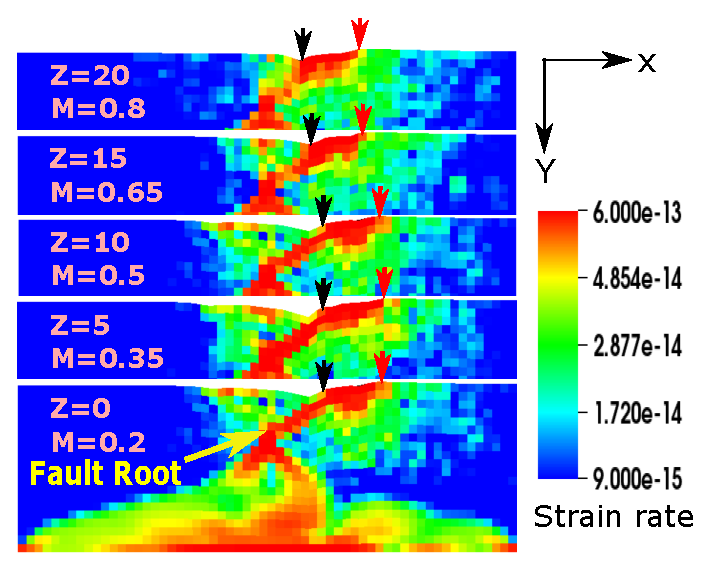
\includegraphics[width=0.6\textwidth]{fig_Results1_2.eps}
  \caption{Strain rate at 107.5kyr with five slices along ridge axis(Z axis).}
 \label{fig_Results1_2}
\end{figure}   

The location of the termination of the detachment fault where footwall begins to be exhumed to the surface varies along the ridge-axis (i.e. Z-axis). As shown in Figure~\ref{fig_Results1_2}, the highest strain rate regions can be interpreted as detachment fault interfaces. When M$<=0.5$, although the fault displacement should be higher for lower M, the rate of bending of the fault has a maximum value controlled by the far field extension rate, thus the faulting interfaces are similar. When M$>0.5$, the displacement as well as the amount of the bending of the fault decrease as M increases which help maintaining a higher angle fault and thus a nearer to the ridge-axis termination. However, this behavior is more or less compensated by the hanging wall being pushed away from the ridge-axis due to excessive diking (when M$>0.5$). In a unit time, the volume of the exhumation is also smaller for the higher M side.       

Corrugations are observed in the model since 240kyr. It will be further discussed in the discussion chapter. There are two contributing factors, for one, trans-extenstional stresses are created due to offset of the breakaway as well as the variation in fault displacements along the ridge axis; for the other, the variation of the position of the termination of the detachment fault might create anastomosing faults mentioned in \citep{Smith2014}.      

The secondary near axis high angle normal fault is another common observation of the models. At the ridge axis with M$>0.5$, (In this reference model, M$=0.5$ is at the center of ther ridge-axis (Z=10).) the existing normal fault will be pushed away from the ridge-axis due to excessive diking, as its mechanism has been mentioned in introduction chapter, another new near axis normal fault is created at around 650kyr. As it evolve, the initial detachment fault become inactive. This secondary fault creates another dome and its composition is more likely to be volcanic rather than ultramafic, however, as is evolve, if it can last long, lower crust and upper mantle material can be exhumed to the surface. The composition of the domes observed at Kane magamullions is similar to this mechanism that ultramafic Babel dome is on the West and crustal inside-corner high on the East.    

\subsubsection{Constant M along the ridge axis }

As shown in Figure~\ref{fig_Results1_3}, the width and depth of the median valley is almost constant. The variation in breakaway and termination as well as the existence of corrugation mentioned in reference model one are not observed. 
\begin{figure}[H]
  \centering
    \includegraphics[width=1.0\textwidth]{fig_Results1_3.eps}
  \caption{Reference model two: constant M$=0.8$ along the ridge-axis (i.e. Z axis). Type two weakening.}
 \label{fig_Results1_3}
\end{figure}   


\subsection{Variation of the range of M}

\


\subsection{Variation of the functional form}

\subsection{Influence of weakening rate}

\subsection{Summary of Findings}

\pagebreak
\section{Discussion}
\subsection{Model Limitation}

\pagebreak
\section{Conclusions}
\remove[EC]{For the first time, we}{I} model in 3D how \remove[EC]{varying} M \remove[EC]{value (magma supply)} \add[EC]{varying} along \change[EC]{the}{a} \remove[EC]{the} mid-ocean ridge segment can control the interaction\add[EC]{s} between tectonics and magmatism and \add[EC]{thereby produce} the major bathymetric features observed on the seafloor.
Six commonly observed MOR features \annote[EC]{(}{STOP USING PARENTHESES LIKE THIS!!!!!!} \remove[EC]{i.e. inward fault jump, fault alternation, mass wasting, hourglass median valley, corrugation and mullion structure)} are produced \change[EC]{by}{in} our model \add[EC]{which are} inward fault jump, fault alternation, mass wasting, hourglass median valley, corrugation, and mullion structure. 
\add[EC]{I show that,} by comparing \add[EC]{these features of} the model\change[EC]{ results}{s} and \add[EC]{those of the} \annote[EC]{local}{What do you mean by ``local''?} field observations, faulting \remove[EC]{evolution} history \change[EC]{as well as}{and} spatial and temporal variation of magma supply can be inferred \add[EC]{for a ridge segment}.

Three controlling parameters are investigated. They are three ranges of M (i.e. M28, M57 and M58); three types of functional forms of M variation (i.e. linear, sinusoidal and sqaure root) as well as two types of weakening rates (i.e. faster type 1 and slower type 2). \change[EC]{As result shows, a}{A}lthough different structural features are generated by different functional forms and ranges of M variations along the ridge, the average M value ($\bar{M}$) along the whole ridge segment \change[EC]{is the major value that is responsible for the two end members of}{controls} off-axis morphologies\change[EC]{, i.e. w}{. W}hen $\bar{M} >$ 0.6425 with type 2 weakening, \change[EC]{the model generates symmetrial spreading, short wavelength abyssal hills}{spreading occurs symmetrically and short-wavelength abyssal hills are produced.} \change[EC]{whereas}{In constrast,} when $\bar{M} \le$ 0.6425, \remove[EC]{faults tend to rotate to a low angle,} \add[EC]{a} long lasting detachment fault \add[EC]{forms,} \change[EC]{that}{which} can exhume ultramafic rocks to the seafloor producing a domal OCC. Also, our 3D model results resolve the discrepancy between previous 2D model studies and field observations that model studies suggest OCC is produced when M varies from 0.3 to 0.5 but field observation reveals cases that OCC forms with observed M beyond both lower and upper limits. \change[EC]{Based on this thesis study, w}{W}e propose a new perspective \remove[EC]{for explaining cases when OCC forms with local M value is lower than 0.3 or higher than 0.5 by} the along ridge coupling \change[EC]{argument}{can explain why OCCs can form for M smaller than 0.3 or greater than 0.5}. \change[EC]{In addition}{Finally}, we propose \change[EC]{a new hypothesis of the asynchronous faulting induced tensile failure as one possible formation mechanism for the enigmatic corrugations widely observed on the surface of OCCs}{that the asynchronous faulting can generate along-ridge tensile stresses of a large enough magnitude to cause tensile failure on the surface of the dome of an OCC, producing corrugations widely observed on the OCCs in nature}.




  % <>? should I use Summary or Conclusions?
%\include{Recommendations} % <>? what is recommendations for?

%%--------------------------------------------------
% Reference Pages
%%--------------------------------------------------

%\include{Glossary}  % optional
%\include{References}
%\include{Appendices}

\bibliographystyle{abbrvnat}
\bibliography{References.bib}

\end{document}
